\documentclass[12pt]{article}

\usepackage[english]{babel}
\usepackage[top=2cm,bottom=2cm,left=2.5cm,right=2.5cm,marginparwidth=1.75cm]{geometry}
\usepackage{setspace}
\usepackage{longtable}
\usepackage{ragged2e}

\usepackage[hidelinks,urlcolor=cyan]{hyperref}
\urlstyle{same}



\setlength{\parindent}{0pt}
\setlength{\parskip}{1ex}

\usepackage{graphicx}
\graphicspath{ {images/} }

\title{Horses in the Industrial Revolution}
\author{Fletcher Gornick}
\date{July 2021}

\addto\captionsenglish{\renewcommand{\contentsname}{Table of Contents}}

\def \n {\par \vspace{1ex}}

\begin{document}
\onehalfspacing
\begin{titlepage}
    \begin{center}
        \vspace*{1cm}
            
        \Huge
        \textbf{Horses in the Industrial Revolution}
            
        \vspace{0.5cm}
        \LARGE
        ANSC 1701, Summer 2021 Semester
            
        \vspace{1.5cm}
            
        \textbf{Fletcher Gornick}
            
        \vfill
            
        Historical Inquiry Document for\\
        Horse History Project
            
        \vspace{0.8cm}
            
        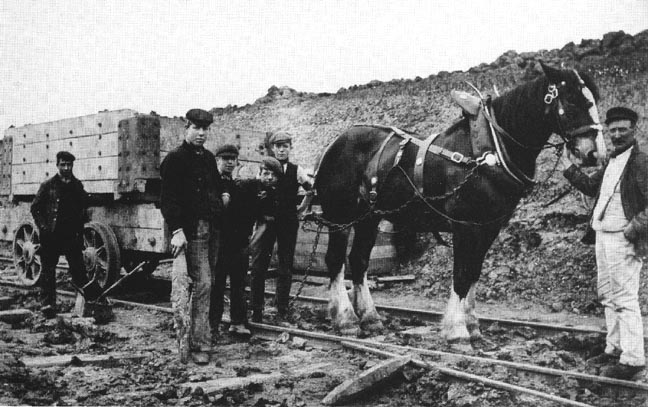
\includegraphics[scale=0.5]{title_horse.jpg}
        
        \vspace{1cm}
        \Large
        University of Minnesota \\
        Department of Animal Science \\
        July 2021
            
    \end{center}
\end{titlepage}

\tableofcontents
\newpage

\section{Selection of Research Topic / Question}
\subsection{Topic}
\textbf{Topic: } Horses in the Industrial Revolution. \\

\textbf{Question: } How has the Industrial Revolution altered the role of horses in agriculture and/or industry during late 18th and early 19th century, and what impact did that have on horses in modern society? \\
\subsection{Analysis of Question}
{\renewcommand{\arraystretch}{2}
\begin{longtable}{ | p{6cm} | p{10cm} | }

\hline
Is the question historical and does it have historical significance? & 

Horses played a key role in our pre-industrialized economy.  They were the main source of transportation and were critical to agriculture, so the impact that the Industrial Revolution had on the horse is very historically significant.
\\\hline

Is the answer to the question obvious or a matter of opinion? & 

No.  The question, while it can be speculated, cannot be answered by a simple search, and The Industrial Revolution had a very concrete impact on the horse, it's not a matter of opinion.
\\\hline

What pieces of information will be needed to provide the framework so that you can infer an answer to the question? & 

1) The role horses played before the Industrial Revolution. \n\n

2) What horses did to contribute to the success of the pre-industrialized economy. \n\n

3) The role horses played after the Industrial Revolution. \n\n

4) Specific aspects of the Industrial Revolution that resulted in this change in roles. \newline
\\\hline

Provide at least 3 potential sources of information. & 

1) 2013 article about the role of horses in brewing during the industrial revolution \cite{almer13}. \n\n

2) 1820 image drawn of a horse hauling a dray (low, flat-bed wagon without sides) \cite{schar20}. \n\n

3) 1982 article written about the British Industrial Revolution \cite{musso82}. \n\n

4) 1831 book containing general history and zoological classification of the horse 
\cite{youat31} \newline
\\\hline

\end{longtable}}

\newpage

\section{Sources of Information}
\textbf{Topic: } Horses in the Industrial Revolution. \\

\textbf{Question: } How has the Industrial Revolution altered the role of horses in agriculture and/or industry during late 18th and early 19th century, and what impact did that have on horses in modern society? \\

\subsection{Classification}
{\renewcommand{\arraystretch}{2}
\begin{longtable}{ | p{2.8cm} | p{1.5cm} | p{1.7cm} | p{10cm} | }
\hline

\RaggedRight \textbf{Sources of Information} & 
Primary & Secondary &
Reason why you classified it as such? \n\n

How does the source relate to your question? \n\n

Location of the source? \newline
\\\hline\hline



\RaggedRight Scholarly article on the importance of the horses in the brewing industry
& & X &
\textbf{Secondary source criteria:} This article was written in 2013, so it's not a firsthand account.  It gathers information about equine power in London around the time period in question. \newline

\textbf{Relevance:} It's an article detailing the importance of the horse in the brewing industry which closely mirrors my topic. \newline

\RaggedRight \textbf{Location:} Research paper written by Thomas Almeroth-Williams: \n
\url{https://www.jstor.org/stable/26398226} \newline
\\\hline



\RaggedRight Page 406 and 407 of \emph{The Horse : With a Treatise on Draught and a Copious Index}
& X & & 
\textbf{Primary source criteria:} Written in 1831, provides plenty of relevant information around the end of the industrial revolution. \newline

\textbf{Relevance:} While not 100\% relevant to the topic of the horse's role in the industrial revolution, the book provide plenty of relevant information on horse's history and relation to us, as well as some important zoological classifications to keep my facts straight. \newline

\textbf{Location:} Published by Baldwin and Cradock, and written in London.  \n

\RaggedRight Found on Biodiversity Heritage Library: \newline
\url{https://archive.org/details/horsewithtreatis00youa/page/n5/mode/2up} \newline
\\\hline



\RaggedRight Painting of carthorse being backed into a dray 
& X & &
\textbf{Primary source criteria:} Painted in 1792 around the start of the industrial revolution. \newline

\textbf{Relevance:} The mill-horse was gradually replaced by steam engine, leading to a higher demand for the dray-horse. \newline

\textbf{Location:} painted engraving of Whitbread Brewery in Chiswell Street London in 1792 by George Garrard. \n

\RaggedRight found on Spartacus Educational: \newline
\url{https://spartacus-educational.com/BUwhitbread.htm} \newline
\\\hline



\RaggedRight Graph of Truman Brewery horse stock showing change of mill-horse and dray-horse use over time
& X & &
\textbf{Primary source criteria:} Graph created in 1790 around the start of the industrial revolution. \newline

\textbf{Relevance:} Same reasoning as previous source, but actually shows statistics of relative decline of mill-horse, and incline of dray-horse. \newline

\textbf{Location:} Created in London and submitted to the London Metropolitan Archives: \n\n

\url{https://horsesrevolution.wordpress.com/} \newline
\\\hline



\RaggedRight Excerpt from Part II of \emph{A Farewell to Alms: A Brief Economic History of the World}
& & X &
\textbf{Secondary source criteria:} Book written in 2007. Gathers information about general history of the Industrial Revolution. \newline

\textbf{Relevance:} Mentions horses' prolonged use in jobs such as transportation even after development of steam engine during industrial revolution. \newline

\RaggedRight \textbf{Location:} Book written by Gregory Clark for the Princeton University Press: \n
\url{http://faculty.econ.ucdavis.edu/faculty/gclark/ecn110b/readings/ecn110b-chapter2-2005.pdf} \newline
\\\hline



\RaggedRight Image of horse-drawn carriage used for early NYC fire department
& & X &
\textbf{Secondary source criteria:} Not during industrial revolution per se, but first hand account of the use of horses almost directly after the industrial revolution. \newline

\textbf{Relevance:} Shows a specific use for horses after the industrial revolution. \newline

\textbf{Location:} Picture taken in New York, in 1887. \n

\RaggedRight Found on archives.org: \newline
\url{https://archive.org/details/ourfiremenhistor00cost/page/n7/mode/1up?view=theater} \newline
\\\hline
\end{longtable}}
\newpage

\subsection{Sources}
\input{sources/source_1}

\textbf{What does this source tell you that would be obvious, as it relates to your question?}
\begin{itemize}
    \item Animals, especially horses, played an important role during the industrial revolution.
    \item The economy of the UK metropolitan area is very dependent on the use of horses in industries such as brewing and alcohol distribution.
    \item Industrial revolution actually led to an increased use of horses in urban cities rather than the expected decrease.
    \\
\end{itemize}

\textbf{What does this source tell you that may not be as obvious?}
\begin{itemize}
    \item The article is pretty clear in what information it displays to the reader without much room for interpretation, but going off just the abstract, there's plenty to learn.
    \item One example is how the industrial revolution actually increased the importance of the horse.  The abstract states that the reliance on horses increased, but failed to mention that it came as a result of the steam engine shifting the jobs of brewing  horses from processing grain, to distributing the finished product.
\end{itemize}

\textbf{What does this source tell you that would be obvious, as it relates to your question?}
\begin{itemize}
    \item Animals, especially horses, played an important role during the industrial revolution.
    \item The economy of the UK metropolitan area is very dependent on the use of horses in industries such as brewing and alcohol distribution.
    \item Industrial revolution actually led to an increased use of horses in urban cities rather than the expected decrease.
    \\
\end{itemize}

\textbf{What does this source tell you that may not be as obvious?}
\begin{itemize}
    \item The article is pretty clear in what information it displays to the reader without much room for interpretation, but going off just the abstract, there's plenty to learn.
    \item One example is how the industrial revolution actually increased the importance of the horse.  The abstract states that the reliance on horses increased, but failed to mention that it came as a result of the steam engine shifting the jobs of brewing  horses from processing grain, to distributing the finished product.
\end{itemize}

\textbf{What does this source tell you that would be obvious, as it relates to your question?}
\begin{itemize}
    \item Animals, especially horses, played an important role during the industrial revolution.
    \item The economy of the UK metropolitan area is very dependent on the use of horses in industries such as brewing and alcohol distribution.
    \item Industrial revolution actually led to an increased use of horses in urban cities rather than the expected decrease.
    \\
\end{itemize}

\textbf{What does this source tell you that may not be as obvious?}
\begin{itemize}
    \item The article is pretty clear in what information it displays to the reader without much room for interpretation, but going off just the abstract, there's plenty to learn.
    \item One example is how the industrial revolution actually increased the importance of the horse.  The abstract states that the reliance on horses increased, but failed to mention that it came as a result of the steam engine shifting the jobs of brewing  horses from processing grain, to distributing the finished product.
\end{itemize} \newpage
\input{sources/source_2}

\textbf{The story this book excerpt tells:} This article compares the cost of using horses vs machinery for railway work.  As the industrial revolution brought forth the steam engine, it became a matter of whether or not the investment of one was worth it.  Especially in it's early stages, the steam engine wasn't nearly as efficient as it is today, so horses were still used for quite a while after the industrial revolution for tasks such as railway work.  The most obvious example from this excerpt explaining this story would be the list of expenses for both the horse and steam engine.  But overall this excerpt basically proves that horses were still quite the necessity even decades after the industrial revolution.

\textbf{The story this book excerpt tells:} This article compares the cost of using horses vs machinery for railway work.  As the industrial revolution brought forth the steam engine, it became a matter of whether or not the investment of one was worth it.  Especially in it's early stages, the steam engine wasn't nearly as efficient as it is today, so horses were still used for quite a while after the industrial revolution for tasks such as railway work.  The most obvious example from this excerpt explaining this story would be the list of expenses for both the horse and steam engine.  But overall this excerpt basically proves that horses were still quite the necessity even decades after the industrial revolution.

\textbf{The story this book excerpt tells:} This article compares the cost of using horses vs machinery for railway work.  As the industrial revolution brought forth the steam engine, it became a matter of whether or not the investment of one was worth it.  Especially in it's early stages, the steam engine wasn't nearly as efficient as it is today, so horses were still used for quite a while after the industrial revolution for tasks such as railway work.  The most obvious example from this excerpt explaining this story would be the list of expenses for both the horse and steam engine.  But overall this excerpt basically proves that horses were still quite the necessity even decades after the industrial revolution.
\input{sources/source_3}

\textbf{The story this painting tells:} This painting's primary purpose was to shed light on what it's like in the London Brewing Industries back in the late 1700s. As to how it relates to my topic of the horses' role after the industrial revolution, this paints a pretty clear picture.  Context of the time tells us that the mill-horse's replacement with the steam engine lead to more horses being used to cart around barrels of beer.  Therefore the horse depicted in this painting is, in part, a consequence of the industrial revolution. Some clues in the painting that indicate this story would obviously be the horse being backed into a dray, some of the barrels of beer you can see in the background, and also the title of the painting "Whitbread Brewery in Chiswell street".  One minor detail that may indirectly show the steam engine taking over the original milling job of the horse would be the smoke clouds in the background.

\textbf{The story this painting tells:} This painting's primary purpose was to shed light on what it's like in the London Brewing Industries back in the late 1700s. As to how it relates to my topic of the horses' role after the industrial revolution, this paints a pretty clear picture.  Context of the time tells us that the mill-horse's replacement with the steam engine lead to more horses being used to cart around barrels of beer.  Therefore the horse depicted in this painting is, in part, a consequence of the industrial revolution. Some clues in the painting that indicate this story would obviously be the horse being backed into a dray, some of the barrels of beer you can see in the background, and also the title of the painting "Whitbread Brewery in Chiswell street".  One minor detail that may indirectly show the steam engine taking over the original milling job of the horse would be the smoke clouds in the background.

\textbf{The story this painting tells:} This painting's primary purpose was to shed light on what it's like in the London Brewing Industries back in the late 1700s. As to how it relates to my topic of the horses' role after the industrial revolution, this paints a pretty clear picture.  Context of the time tells us that the mill-horse's replacement with the steam engine lead to more horses being used to cart around barrels of beer.  Therefore the horse depicted in this painting is, in part, a consequence of the industrial revolution. Some clues in the painting that indicate this story would obviously be the horse being backed into a dray, some of the barrels of beer you can see in the background, and also the title of the painting "Whitbread Brewery in Chiswell street".  One minor detail that may indirectly show the steam engine taking over the original milling job of the horse would be the smoke clouds in the background. \newpage
{\renewcommand{\arraystretch}{2}
\begin{longtable}{ | p{3cm} | p{13cm} | }
\hline

\textbf{Source 4} &
Graph of the Truman Brewery horse stock over time
\\\hline

\textbf{Subject} &
The graph depicts a the population of both the mill-horse and dray horse.  Shows how around the time the steam engine was developed, the relative population of the mill-horse decreased, while the dray-horse population increased.
\\\hline

\textbf{Author} &
\textbf{Name:} Unknown \n

\textbf{Point of View:} Statistician  working in the London metropolitan area gathering information about brewing industries
\\\hline

\textbf{Production} &
\textbf{When was the source produced:} Graphed in 1759

\textbf{Where was the source produced:} London, UK \n

\textbf{What was happening within the immediate and broader context at the time the source was produced, as it relates to the source? } \n

This graph, just like the painting in Source 3 was made around the time the mill-horse was rendered obsolete by the steam engine.  This graph was most likely made to provide a sort of explanation as to why these horse populations were changing.
\\\hline

\textbf{Audience} &
\textbf{Who was the intended audience?} Other statisticians or brewery owners \n 

\textbf{Was it meant to be persuasive to a particular point of view? } \n

This graph is sheerly informational, and meant to graph the correlation between the rise of the steam engine and the relative population of certain horses.  Therefore this is not meant to persuade, it's instead meant to inform
\\\hline
\end{longtable}} \newpage
\input{sources/source_5}

\textbf{What does this source tell you that would be obvious, as it relates to your question?}
\begin{itemize}
    \item The creation of the steam powered railway lead to 6000 miles of track being laid down in only 26 years.
    \item Horses were used to pull coal carts on tram lines out of mines for carriage to London.  This was before the development of the steam engine.
    \item Since the Watt steam engine was so heavy, it didn't take over the industry for a while, as the cost to use the engine outweighed the profit from the transported coal. 
    \\
\end{itemize}

\textbf{What does this source tell you that may not be as obvious?}
\begin{itemize}
    \item It was the development of the high-pressure steam engine that sparked the widespread use of machinery in place of horses for tasks such as moving coal.
    \item Even after the development of the high pressure steam engine, horses were still an important factor in the growth of Great Britain.
\end{itemize}

\textbf{What does this source tell you that would be obvious, as it relates to your question?}
\begin{itemize}
    \item The creation of the steam powered railway lead to 6000 miles of track being laid down in only 26 years.
    \item Horses were used to pull coal carts on tram lines out of mines for carriage to London.  This was before the development of the steam engine.
    \item Since the Watt steam engine was so heavy, it didn't take over the industry for a while, as the cost to use the engine outweighed the profit from the transported coal. 
    \\
\end{itemize}

\textbf{What does this source tell you that may not be as obvious?}
\begin{itemize}
    \item It was the development of the high-pressure steam engine that sparked the widespread use of machinery in place of horses for tasks such as moving coal.
    \item Even after the development of the high pressure steam engine, horses were still an important factor in the growth of Great Britain.
\end{itemize}

\textbf{What does this source tell you that would be obvious, as it relates to your question?}
\begin{itemize}
    \item The creation of the steam powered railway lead to 6000 miles of track being laid down in only 26 years.
    \item Horses were used to pull coal carts on tram lines out of mines for carriage to London.  This was before the development of the steam engine.
    \item Since the Watt steam engine was so heavy, it didn't take over the industry for a while, as the cost to use the engine outweighed the profit from the transported coal. 
    \\
\end{itemize}

\textbf{What does this source tell you that may not be as obvious?}
\begin{itemize}
    \item It was the development of the high-pressure steam engine that sparked the widespread use of machinery in place of horses for tasks such as moving coal.
    \item Even after the development of the high pressure steam engine, horses were still an important factor in the growth of Great Britain.
\end{itemize} \newpage
\input{sources/source_6}

\textbf{What does this source tell you that would be obvious, as it relates to your question?}
\begin{itemize}
    \item In the early NYC fire department, horses were used to transport firemen within the city.
    \item All this source really shows is a horse pulling a cart with some official looking people, most likely for the purpose of something important.
    \\
\end{itemize}

\textbf{What does this source tell you that may not be as obvious?}
\begin{itemize}
    \item The picture itself actually comes from a biographical book about firemen.
    \item This book brings up a detailed history of the early days of the New York City Fire Department, as well as their reliance on animals such as horses for quick inner-city travel.
\end{itemize}

\textbf{What does this source tell you that would be obvious, as it relates to your question?}
\begin{itemize}
    \item In the early NYC fire department, horses were used to transport firemen within the city.
    \item All this source really shows is a horse pulling a cart with some official looking people, most likely for the purpose of something important.
    \\
\end{itemize}

\textbf{What does this source tell you that may not be as obvious?}
\begin{itemize}
    \item The picture itself actually comes from a biographical book about firemen.
    \item This book brings up a detailed history of the early days of the New York City Fire Department, as well as their reliance on animals such as horses for quick inner-city travel.
\end{itemize}

\textbf{What does this source tell you that would be obvious, as it relates to your question?}
\begin{itemize}
    \item In the early NYC fire department, horses were used to transport firemen within the city.
    \item All this source really shows is a horse pulling a cart with some official looking people, most likely for the purpose of something important.
    \\
\end{itemize}

\textbf{What does this source tell you that may not be as obvious?}
\begin{itemize}
    \item The picture itself actually comes from a biographical book about firemen.
    \item This book brings up a detailed history of the early days of the New York City Fire Department, as well as their reliance on animals such as horses for quick inner-city travel.
\end{itemize} \newpage

\section{Contextualizing Research Sources}
\textbf{Topic: } Horses in the Industrial Revolution. \\

\textbf{Question: } How has the Industrial Revolution altered the role of horses in agriculture and/or industry during late 18th and early 19th century, and what impact did that have on horses in modern society? \\
\input{sources/source_1}

\textbf{What does this source tell you that would be obvious, as it relates to your question?}
\begin{itemize}
    \item Animals, especially horses, played an important role during the industrial revolution.
    \item The economy of the UK metropolitan area is very dependent on the use of horses in industries such as brewing and alcohol distribution.
    \item Industrial revolution actually led to an increased use of horses in urban cities rather than the expected decrease.
    \\
\end{itemize}

\textbf{What does this source tell you that may not be as obvious?}
\begin{itemize}
    \item The article is pretty clear in what information it displays to the reader without much room for interpretation, but going off just the abstract, there's plenty to learn.
    \item One example is how the industrial revolution actually increased the importance of the horse.  The abstract states that the reliance on horses increased, but failed to mention that it came as a result of the steam engine shifting the jobs of brewing  horses from processing grain, to distributing the finished product.
\end{itemize}

\textbf{What does this source tell you that would be obvious, as it relates to your question?}
\begin{itemize}
    \item Animals, especially horses, played an important role during the industrial revolution.
    \item The economy of the UK metropolitan area is very dependent on the use of horses in industries such as brewing and alcohol distribution.
    \item Industrial revolution actually led to an increased use of horses in urban cities rather than the expected decrease.
    \\
\end{itemize}

\textbf{What does this source tell you that may not be as obvious?}
\begin{itemize}
    \item The article is pretty clear in what information it displays to the reader without much room for interpretation, but going off just the abstract, there's plenty to learn.
    \item One example is how the industrial revolution actually increased the importance of the horse.  The abstract states that the reliance on horses increased, but failed to mention that it came as a result of the steam engine shifting the jobs of brewing  horses from processing grain, to distributing the finished product.
\end{itemize}

\textbf{What does this source tell you that would be obvious, as it relates to your question?}
\begin{itemize}
    \item Animals, especially horses, played an important role during the industrial revolution.
    \item The economy of the UK metropolitan area is very dependent on the use of horses in industries such as brewing and alcohol distribution.
    \item Industrial revolution actually led to an increased use of horses in urban cities rather than the expected decrease.
    \\
\end{itemize}

\textbf{What does this source tell you that may not be as obvious?}
\begin{itemize}
    \item The article is pretty clear in what information it displays to the reader without much room for interpretation, but going off just the abstract, there's plenty to learn.
    \item One example is how the industrial revolution actually increased the importance of the horse.  The abstract states that the reliance on horses increased, but failed to mention that it came as a result of the steam engine shifting the jobs of brewing  horses from processing grain, to distributing the finished product.
\end{itemize} \newpage
\input{sources/source_2}

\textbf{The story this book excerpt tells:} This article compares the cost of using horses vs machinery for railway work.  As the industrial revolution brought forth the steam engine, it became a matter of whether or not the investment of one was worth it.  Especially in it's early stages, the steam engine wasn't nearly as efficient as it is today, so horses were still used for quite a while after the industrial revolution for tasks such as railway work.  The most obvious example from this excerpt explaining this story would be the list of expenses for both the horse and steam engine.  But overall this excerpt basically proves that horses were still quite the necessity even decades after the industrial revolution.

\textbf{The story this book excerpt tells:} This article compares the cost of using horses vs machinery for railway work.  As the industrial revolution brought forth the steam engine, it became a matter of whether or not the investment of one was worth it.  Especially in it's early stages, the steam engine wasn't nearly as efficient as it is today, so horses were still used for quite a while after the industrial revolution for tasks such as railway work.  The most obvious example from this excerpt explaining this story would be the list of expenses for both the horse and steam engine.  But overall this excerpt basically proves that horses were still quite the necessity even decades after the industrial revolution.

\textbf{The story this book excerpt tells:} This article compares the cost of using horses vs machinery for railway work.  As the industrial revolution brought forth the steam engine, it became a matter of whether or not the investment of one was worth it.  Especially in it's early stages, the steam engine wasn't nearly as efficient as it is today, so horses were still used for quite a while after the industrial revolution for tasks such as railway work.  The most obvious example from this excerpt explaining this story would be the list of expenses for both the horse and steam engine.  But overall this excerpt basically proves that horses were still quite the necessity even decades after the industrial revolution. \newpage
\input{sources/source_3}

\textbf{The story this painting tells:} This painting's primary purpose was to shed light on what it's like in the London Brewing Industries back in the late 1700s. As to how it relates to my topic of the horses' role after the industrial revolution, this paints a pretty clear picture.  Context of the time tells us that the mill-horse's replacement with the steam engine lead to more horses being used to cart around barrels of beer.  Therefore the horse depicted in this painting is, in part, a consequence of the industrial revolution. Some clues in the painting that indicate this story would obviously be the horse being backed into a dray, some of the barrels of beer you can see in the background, and also the title of the painting "Whitbread Brewery in Chiswell street".  One minor detail that may indirectly show the steam engine taking over the original milling job of the horse would be the smoke clouds in the background.

\textbf{The story this painting tells:} This painting's primary purpose was to shed light on what it's like in the London Brewing Industries back in the late 1700s. As to how it relates to my topic of the horses' role after the industrial revolution, this paints a pretty clear picture.  Context of the time tells us that the mill-horse's replacement with the steam engine lead to more horses being used to cart around barrels of beer.  Therefore the horse depicted in this painting is, in part, a consequence of the industrial revolution. Some clues in the painting that indicate this story would obviously be the horse being backed into a dray, some of the barrels of beer you can see in the background, and also the title of the painting "Whitbread Brewery in Chiswell street".  One minor detail that may indirectly show the steam engine taking over the original milling job of the horse would be the smoke clouds in the background.

\textbf{The story this painting tells:} This painting's primary purpose was to shed light on what it's like in the London Brewing Industries back in the late 1700s. As to how it relates to my topic of the horses' role after the industrial revolution, this paints a pretty clear picture.  Context of the time tells us that the mill-horse's replacement with the steam engine lead to more horses being used to cart around barrels of beer.  Therefore the horse depicted in this painting is, in part, a consequence of the industrial revolution. Some clues in the painting that indicate this story would obviously be the horse being backed into a dray, some of the barrels of beer you can see in the background, and also the title of the painting "Whitbread Brewery in Chiswell street".  One minor detail that may indirectly show the steam engine taking over the original milling job of the horse would be the smoke clouds in the background. \newpage
{\renewcommand{\arraystretch}{2}
\begin{longtable}{ | p{3cm} | p{13cm} | }
\hline

\textbf{Source 4} &
Graph of the Truman Brewery horse stock over time
\\\hline

\textbf{Subject} &
The graph depicts a the population of both the mill-horse and dray horse.  Shows how around the time the steam engine was developed, the relative population of the mill-horse decreased, while the dray-horse population increased.
\\\hline

\textbf{Author} &
\textbf{Name:} Unknown \n

\textbf{Point of View:} Statistician  working in the London metropolitan area gathering information about brewing industries
\\\hline

\textbf{Production} &
\textbf{When was the source produced:} Graphed in 1759

\textbf{Where was the source produced:} London, UK \n

\textbf{What was happening within the immediate and broader context at the time the source was produced, as it relates to the source? } \n

This graph, just like the painting in Source 3 was made around the time the mill-horse was rendered obsolete by the steam engine.  This graph was most likely made to provide a sort of explanation as to why these horse populations were changing.
\\\hline

\textbf{Audience} &
\textbf{Who was the intended audience?} Other statisticians or brewery owners \n 

\textbf{Was it meant to be persuasive to a particular point of view? } \n

This graph is sheerly informational, and meant to graph the correlation between the rise of the steam engine and the relative population of certain horses.  Therefore this is not meant to persuade, it's instead meant to inform
\\\hline
\end{longtable}} \newpage
\input{sources/source_5}

\textbf{What does this source tell you that would be obvious, as it relates to your question?}
\begin{itemize}
    \item The creation of the steam powered railway lead to 6000 miles of track being laid down in only 26 years.
    \item Horses were used to pull coal carts on tram lines out of mines for carriage to London.  This was before the development of the steam engine.
    \item Since the Watt steam engine was so heavy, it didn't take over the industry for a while, as the cost to use the engine outweighed the profit from the transported coal. 
    \\
\end{itemize}

\textbf{What does this source tell you that may not be as obvious?}
\begin{itemize}
    \item It was the development of the high-pressure steam engine that sparked the widespread use of machinery in place of horses for tasks such as moving coal.
    \item Even after the development of the high pressure steam engine, horses were still an important factor in the growth of Great Britain.
\end{itemize}

\textbf{What does this source tell you that would be obvious, as it relates to your question?}
\begin{itemize}
    \item The creation of the steam powered railway lead to 6000 miles of track being laid down in only 26 years.
    \item Horses were used to pull coal carts on tram lines out of mines for carriage to London.  This was before the development of the steam engine.
    \item Since the Watt steam engine was so heavy, it didn't take over the industry for a while, as the cost to use the engine outweighed the profit from the transported coal. 
    \\
\end{itemize}

\textbf{What does this source tell you that may not be as obvious?}
\begin{itemize}
    \item It was the development of the high-pressure steam engine that sparked the widespread use of machinery in place of horses for tasks such as moving coal.
    \item Even after the development of the high pressure steam engine, horses were still an important factor in the growth of Great Britain.
\end{itemize}

\textbf{What does this source tell you that would be obvious, as it relates to your question?}
\begin{itemize}
    \item The creation of the steam powered railway lead to 6000 miles of track being laid down in only 26 years.
    \item Horses were used to pull coal carts on tram lines out of mines for carriage to London.  This was before the development of the steam engine.
    \item Since the Watt steam engine was so heavy, it didn't take over the industry for a while, as the cost to use the engine outweighed the profit from the transported coal. 
    \\
\end{itemize}

\textbf{What does this source tell you that may not be as obvious?}
\begin{itemize}
    \item It was the development of the high-pressure steam engine that sparked the widespread use of machinery in place of horses for tasks such as moving coal.
    \item Even after the development of the high pressure steam engine, horses were still an important factor in the growth of Great Britain.
\end{itemize} \newpage
\input{sources/source_6}

\textbf{What does this source tell you that would be obvious, as it relates to your question?}
\begin{itemize}
    \item In the early NYC fire department, horses were used to transport firemen within the city.
    \item All this source really shows is a horse pulling a cart with some official looking people, most likely for the purpose of something important.
    \\
\end{itemize}

\textbf{What does this source tell you that may not be as obvious?}
\begin{itemize}
    \item The picture itself actually comes from a biographical book about firemen.
    \item This book brings up a detailed history of the early days of the New York City Fire Department, as well as their reliance on animals such as horses for quick inner-city travel.
\end{itemize}

\textbf{What does this source tell you that would be obvious, as it relates to your question?}
\begin{itemize}
    \item In the early NYC fire department, horses were used to transport firemen within the city.
    \item All this source really shows is a horse pulling a cart with some official looking people, most likely for the purpose of something important.
    \\
\end{itemize}

\textbf{What does this source tell you that may not be as obvious?}
\begin{itemize}
    \item The picture itself actually comes from a biographical book about firemen.
    \item This book brings up a detailed history of the early days of the New York City Fire Department, as well as their reliance on animals such as horses for quick inner-city travel.
\end{itemize}

\textbf{What does this source tell you that would be obvious, as it relates to your question?}
\begin{itemize}
    \item In the early NYC fire department, horses were used to transport firemen within the city.
    \item All this source really shows is a horse pulling a cart with some official looking people, most likely for the purpose of something important.
    \\
\end{itemize}

\textbf{What does this source tell you that may not be as obvious?}
\begin{itemize}
    \item The picture itself actually comes from a biographical book about firemen.
    \item This book brings up a detailed history of the early days of the New York City Fire Department, as well as their reliance on animals such as horses for quick inner-city travel.
\end{itemize} \newpage

\section{Evaluating and Analyzing Sources}
\textbf{Topic: } Horses in the Industrial Revolution. \\

\textbf{Question: } How has the Industrial Revolution altered the role of horses in agriculture and/or industry during late 18th and early 19th century, and what impact did that have on horses in modern society? \\

\input{sources/source_1}

\textbf{What does this source tell you that would be obvious, as it relates to your question?}
\begin{itemize}
    \item Animals, especially horses, played an important role during the industrial revolution.
    \item The economy of the UK metropolitan area is very dependent on the use of horses in industries such as brewing and alcohol distribution.
    \item Industrial revolution actually led to an increased use of horses in urban cities rather than the expected decrease.
    \\
\end{itemize}

\textbf{What does this source tell you that may not be as obvious?}
\begin{itemize}
    \item The article is pretty clear in what information it displays to the reader without much room for interpretation, but going off just the abstract, there's plenty to learn.
    \item One example is how the industrial revolution actually increased the importance of the horse.  The abstract states that the reliance on horses increased, but failed to mention that it came as a result of the steam engine shifting the jobs of brewing  horses from processing grain, to distributing the finished product.
\end{itemize}

\textbf{What does this source tell you that would be obvious, as it relates to your question?}
\begin{itemize}
    \item Animals, especially horses, played an important role during the industrial revolution.
    \item The economy of the UK metropolitan area is very dependent on the use of horses in industries such as brewing and alcohol distribution.
    \item Industrial revolution actually led to an increased use of horses in urban cities rather than the expected decrease.
    \\
\end{itemize}

\textbf{What does this source tell you that may not be as obvious?}
\begin{itemize}
    \item The article is pretty clear in what information it displays to the reader without much room for interpretation, but going off just the abstract, there's plenty to learn.
    \item One example is how the industrial revolution actually increased the importance of the horse.  The abstract states that the reliance on horses increased, but failed to mention that it came as a result of the steam engine shifting the jobs of brewing  horses from processing grain, to distributing the finished product.
\end{itemize}

\textbf{What does this source tell you that would be obvious, as it relates to your question?}
\begin{itemize}
    \item Animals, especially horses, played an important role during the industrial revolution.
    \item The economy of the UK metropolitan area is very dependent on the use of horses in industries such as brewing and alcohol distribution.
    \item Industrial revolution actually led to an increased use of horses in urban cities rather than the expected decrease.
    \\
\end{itemize}

\textbf{What does this source tell you that may not be as obvious?}
\begin{itemize}
    \item The article is pretty clear in what information it displays to the reader without much room for interpretation, but going off just the abstract, there's plenty to learn.
    \item One example is how the industrial revolution actually increased the importance of the horse.  The abstract states that the reliance on horses increased, but failed to mention that it came as a result of the steam engine shifting the jobs of brewing  horses from processing grain, to distributing the finished product.
\end{itemize} \newpage
\input{sources/source_2}

\textbf{The story this book excerpt tells:} This article compares the cost of using horses vs machinery for railway work.  As the industrial revolution brought forth the steam engine, it became a matter of whether or not the investment of one was worth it.  Especially in it's early stages, the steam engine wasn't nearly as efficient as it is today, so horses were still used for quite a while after the industrial revolution for tasks such as railway work.  The most obvious example from this excerpt explaining this story would be the list of expenses for both the horse and steam engine.  But overall this excerpt basically proves that horses were still quite the necessity even decades after the industrial revolution.

\textbf{The story this book excerpt tells:} This article compares the cost of using horses vs machinery for railway work.  As the industrial revolution brought forth the steam engine, it became a matter of whether or not the investment of one was worth it.  Especially in it's early stages, the steam engine wasn't nearly as efficient as it is today, so horses were still used for quite a while after the industrial revolution for tasks such as railway work.  The most obvious example from this excerpt explaining this story would be the list of expenses for both the horse and steam engine.  But overall this excerpt basically proves that horses were still quite the necessity even decades after the industrial revolution.

\textbf{The story this book excerpt tells:} This article compares the cost of using horses vs machinery for railway work.  As the industrial revolution brought forth the steam engine, it became a matter of whether or not the investment of one was worth it.  Especially in it's early stages, the steam engine wasn't nearly as efficient as it is today, so horses were still used for quite a while after the industrial revolution for tasks such as railway work.  The most obvious example from this excerpt explaining this story would be the list of expenses for both the horse and steam engine.  But overall this excerpt basically proves that horses were still quite the necessity even decades after the industrial revolution. \newpage
\input{sources/source_3}

\textbf{The story this painting tells:} This painting's primary purpose was to shed light on what it's like in the London Brewing Industries back in the late 1700s. As to how it relates to my topic of the horses' role after the industrial revolution, this paints a pretty clear picture.  Context of the time tells us that the mill-horse's replacement with the steam engine lead to more horses being used to cart around barrels of beer.  Therefore the horse depicted in this painting is, in part, a consequence of the industrial revolution. Some clues in the painting that indicate this story would obviously be the horse being backed into a dray, some of the barrels of beer you can see in the background, and also the title of the painting "Whitbread Brewery in Chiswell street".  One minor detail that may indirectly show the steam engine taking over the original milling job of the horse would be the smoke clouds in the background.

\textbf{The story this painting tells:} This painting's primary purpose was to shed light on what it's like in the London Brewing Industries back in the late 1700s. As to how it relates to my topic of the horses' role after the industrial revolution, this paints a pretty clear picture.  Context of the time tells us that the mill-horse's replacement with the steam engine lead to more horses being used to cart around barrels of beer.  Therefore the horse depicted in this painting is, in part, a consequence of the industrial revolution. Some clues in the painting that indicate this story would obviously be the horse being backed into a dray, some of the barrels of beer you can see in the background, and also the title of the painting "Whitbread Brewery in Chiswell street".  One minor detail that may indirectly show the steam engine taking over the original milling job of the horse would be the smoke clouds in the background.

\textbf{The story this painting tells:} This painting's primary purpose was to shed light on what it's like in the London Brewing Industries back in the late 1700s. As to how it relates to my topic of the horses' role after the industrial revolution, this paints a pretty clear picture.  Context of the time tells us that the mill-horse's replacement with the steam engine lead to more horses being used to cart around barrels of beer.  Therefore the horse depicted in this painting is, in part, a consequence of the industrial revolution. Some clues in the painting that indicate this story would obviously be the horse being backed into a dray, some of the barrels of beer you can see in the background, and also the title of the painting "Whitbread Brewery in Chiswell street".  One minor detail that may indirectly show the steam engine taking over the original milling job of the horse would be the smoke clouds in the background. \newpage
{\renewcommand{\arraystretch}{2}
\begin{longtable}{ | p{3cm} | p{13cm} | }
\hline

\textbf{Source 4} &
Graph of the Truman Brewery horse stock over time
\\\hline

\textbf{Subject} &
The graph depicts a the population of both the mill-horse and dray horse.  Shows how around the time the steam engine was developed, the relative population of the mill-horse decreased, while the dray-horse population increased.
\\\hline

\textbf{Author} &
\textbf{Name:} Unknown \n

\textbf{Point of View:} Statistician  working in the London metropolitan area gathering information about brewing industries
\\\hline

\textbf{Production} &
\textbf{When was the source produced:} Graphed in 1759

\textbf{Where was the source produced:} London, UK \n

\textbf{What was happening within the immediate and broader context at the time the source was produced, as it relates to the source? } \n

This graph, just like the painting in Source 3 was made around the time the mill-horse was rendered obsolete by the steam engine.  This graph was most likely made to provide a sort of explanation as to why these horse populations were changing.
\\\hline

\textbf{Audience} &
\textbf{Who was the intended audience?} Other statisticians or brewery owners \n 

\textbf{Was it meant to be persuasive to a particular point of view? } \n

This graph is sheerly informational, and meant to graph the correlation between the rise of the steam engine and the relative population of certain horses.  Therefore this is not meant to persuade, it's instead meant to inform
\\\hline
\end{longtable}} \newpage
\input{sources/source_5}

\textbf{What does this source tell you that would be obvious, as it relates to your question?}
\begin{itemize}
    \item The creation of the steam powered railway lead to 6000 miles of track being laid down in only 26 years.
    \item Horses were used to pull coal carts on tram lines out of mines for carriage to London.  This was before the development of the steam engine.
    \item Since the Watt steam engine was so heavy, it didn't take over the industry for a while, as the cost to use the engine outweighed the profit from the transported coal. 
    \\
\end{itemize}

\textbf{What does this source tell you that may not be as obvious?}
\begin{itemize}
    \item It was the development of the high-pressure steam engine that sparked the widespread use of machinery in place of horses for tasks such as moving coal.
    \item Even after the development of the high pressure steam engine, horses were still an important factor in the growth of Great Britain.
\end{itemize}

\textbf{What does this source tell you that would be obvious, as it relates to your question?}
\begin{itemize}
    \item The creation of the steam powered railway lead to 6000 miles of track being laid down in only 26 years.
    \item Horses were used to pull coal carts on tram lines out of mines for carriage to London.  This was before the development of the steam engine.
    \item Since the Watt steam engine was so heavy, it didn't take over the industry for a while, as the cost to use the engine outweighed the profit from the transported coal. 
    \\
\end{itemize}

\textbf{What does this source tell you that may not be as obvious?}
\begin{itemize}
    \item It was the development of the high-pressure steam engine that sparked the widespread use of machinery in place of horses for tasks such as moving coal.
    \item Even after the development of the high pressure steam engine, horses were still an important factor in the growth of Great Britain.
\end{itemize}

\textbf{What does this source tell you that would be obvious, as it relates to your question?}
\begin{itemize}
    \item The creation of the steam powered railway lead to 6000 miles of track being laid down in only 26 years.
    \item Horses were used to pull coal carts on tram lines out of mines for carriage to London.  This was before the development of the steam engine.
    \item Since the Watt steam engine was so heavy, it didn't take over the industry for a while, as the cost to use the engine outweighed the profit from the transported coal. 
    \\
\end{itemize}

\textbf{What does this source tell you that may not be as obvious?}
\begin{itemize}
    \item It was the development of the high-pressure steam engine that sparked the widespread use of machinery in place of horses for tasks such as moving coal.
    \item Even after the development of the high pressure steam engine, horses were still an important factor in the growth of Great Britain.
\end{itemize} \newpage
\input{sources/source_6}

\textbf{What does this source tell you that would be obvious, as it relates to your question?}
\begin{itemize}
    \item In the early NYC fire department, horses were used to transport firemen within the city.
    \item All this source really shows is a horse pulling a cart with some official looking people, most likely for the purpose of something important.
    \\
\end{itemize}

\textbf{What does this source tell you that may not be as obvious?}
\begin{itemize}
    \item The picture itself actually comes from a biographical book about firemen.
    \item This book brings up a detailed history of the early days of the New York City Fire Department, as well as their reliance on animals such as horses for quick inner-city travel.
\end{itemize}

\textbf{What does this source tell you that would be obvious, as it relates to your question?}
\begin{itemize}
    \item In the early NYC fire department, horses were used to transport firemen within the city.
    \item All this source really shows is a horse pulling a cart with some official looking people, most likely for the purpose of something important.
    \\
\end{itemize}

\textbf{What does this source tell you that may not be as obvious?}
\begin{itemize}
    \item The picture itself actually comes from a biographical book about firemen.
    \item This book brings up a detailed history of the early days of the New York City Fire Department, as well as their reliance on animals such as horses for quick inner-city travel.
\end{itemize}

\textbf{What does this source tell you that would be obvious, as it relates to your question?}
\begin{itemize}
    \item In the early NYC fire department, horses were used to transport firemen within the city.
    \item All this source really shows is a horse pulling a cart with some official looking people, most likely for the purpose of something important.
    \\
\end{itemize}

\textbf{What does this source tell you that may not be as obvious?}
\begin{itemize}
    \item The picture itself actually comes from a biographical book about firemen.
    \item This book brings up a detailed history of the early days of the New York City Fire Department, as well as their reliance on animals such as horses for quick inner-city travel.
\end{itemize} \newpage

\section{Summarizing Sources}
\textbf{Topic: } Horses in the Industrial Revolution. \\

\textbf{Question: } How has the Industrial Revolution altered the role of horses in agriculture and/or industry during late 18th and early 19th century, and what impact did that have on horses in modern society? \\ \\
\input{sources/source_1}

\textbf{What does this source tell you that would be obvious, as it relates to your question?}
\begin{itemize}
    \item Animals, especially horses, played an important role during the industrial revolution.
    \item The economy of the UK metropolitan area is very dependent on the use of horses in industries such as brewing and alcohol distribution.
    \item Industrial revolution actually led to an increased use of horses in urban cities rather than the expected decrease.
    \\
\end{itemize}

\textbf{What does this source tell you that may not be as obvious?}
\begin{itemize}
    \item The article is pretty clear in what information it displays to the reader without much room for interpretation, but going off just the abstract, there's plenty to learn.
    \item One example is how the industrial revolution actually increased the importance of the horse.  The abstract states that the reliance on horses increased, but failed to mention that it came as a result of the steam engine shifting the jobs of brewing  horses from processing grain, to distributing the finished product.
\end{itemize}

\textbf{What does this source tell you that would be obvious, as it relates to your question?}
\begin{itemize}
    \item Animals, especially horses, played an important role during the industrial revolution.
    \item The economy of the UK metropolitan area is very dependent on the use of horses in industries such as brewing and alcohol distribution.
    \item Industrial revolution actually led to an increased use of horses in urban cities rather than the expected decrease.
    \\
\end{itemize}

\textbf{What does this source tell you that may not be as obvious?}
\begin{itemize}
    \item The article is pretty clear in what information it displays to the reader without much room for interpretation, but going off just the abstract, there's plenty to learn.
    \item One example is how the industrial revolution actually increased the importance of the horse.  The abstract states that the reliance on horses increased, but failed to mention that it came as a result of the steam engine shifting the jobs of brewing  horses from processing grain, to distributing the finished product.
\end{itemize}

\textbf{What does this source tell you that would be obvious, as it relates to your question?}
\begin{itemize}
    \item Animals, especially horses, played an important role during the industrial revolution.
    \item The economy of the UK metropolitan area is very dependent on the use of horses in industries such as brewing and alcohol distribution.
    \item Industrial revolution actually led to an increased use of horses in urban cities rather than the expected decrease.
    \\
\end{itemize}

\textbf{What does this source tell you that may not be as obvious?}
\begin{itemize}
    \item The article is pretty clear in what information it displays to the reader without much room for interpretation, but going off just the abstract, there's plenty to learn.
    \item One example is how the industrial revolution actually increased the importance of the horse.  The abstract states that the reliance on horses increased, but failed to mention that it came as a result of the steam engine shifting the jobs of brewing  horses from processing grain, to distributing the finished product.
\end{itemize} \newpage
\input{sources/source_2}

\textbf{The story this book excerpt tells:} This article compares the cost of using horses vs machinery for railway work.  As the industrial revolution brought forth the steam engine, it became a matter of whether or not the investment of one was worth it.  Especially in it's early stages, the steam engine wasn't nearly as efficient as it is today, so horses were still used for quite a while after the industrial revolution for tasks such as railway work.  The most obvious example from this excerpt explaining this story would be the list of expenses for both the horse and steam engine.  But overall this excerpt basically proves that horses were still quite the necessity even decades after the industrial revolution.

\textbf{The story this book excerpt tells:} This article compares the cost of using horses vs machinery for railway work.  As the industrial revolution brought forth the steam engine, it became a matter of whether or not the investment of one was worth it.  Especially in it's early stages, the steam engine wasn't nearly as efficient as it is today, so horses were still used for quite a while after the industrial revolution for tasks such as railway work.  The most obvious example from this excerpt explaining this story would be the list of expenses for both the horse and steam engine.  But overall this excerpt basically proves that horses were still quite the necessity even decades after the industrial revolution.

\textbf{The story this book excerpt tells:} This article compares the cost of using horses vs machinery for railway work.  As the industrial revolution brought forth the steam engine, it became a matter of whether or not the investment of one was worth it.  Especially in it's early stages, the steam engine wasn't nearly as efficient as it is today, so horses were still used for quite a while after the industrial revolution for tasks such as railway work.  The most obvious example from this excerpt explaining this story would be the list of expenses for both the horse and steam engine.  But overall this excerpt basically proves that horses were still quite the necessity even decades after the industrial revolution. \newpage
\input{sources/source_3}

\textbf{The story this painting tells:} This painting's primary purpose was to shed light on what it's like in the London Brewing Industries back in the late 1700s. As to how it relates to my topic of the horses' role after the industrial revolution, this paints a pretty clear picture.  Context of the time tells us that the mill-horse's replacement with the steam engine lead to more horses being used to cart around barrels of beer.  Therefore the horse depicted in this painting is, in part, a consequence of the industrial revolution. Some clues in the painting that indicate this story would obviously be the horse being backed into a dray, some of the barrels of beer you can see in the background, and also the title of the painting "Whitbread Brewery in Chiswell street".  One minor detail that may indirectly show the steam engine taking over the original milling job of the horse would be the smoke clouds in the background.

\textbf{The story this painting tells:} This painting's primary purpose was to shed light on what it's like in the London Brewing Industries back in the late 1700s. As to how it relates to my topic of the horses' role after the industrial revolution, this paints a pretty clear picture.  Context of the time tells us that the mill-horse's replacement with the steam engine lead to more horses being used to cart around barrels of beer.  Therefore the horse depicted in this painting is, in part, a consequence of the industrial revolution. Some clues in the painting that indicate this story would obviously be the horse being backed into a dray, some of the barrels of beer you can see in the background, and also the title of the painting "Whitbread Brewery in Chiswell street".  One minor detail that may indirectly show the steam engine taking over the original milling job of the horse would be the smoke clouds in the background.

\textbf{The story this painting tells:} This painting's primary purpose was to shed light on what it's like in the London Brewing Industries back in the late 1700s. As to how it relates to my topic of the horses' role after the industrial revolution, this paints a pretty clear picture.  Context of the time tells us that the mill-horse's replacement with the steam engine lead to more horses being used to cart around barrels of beer.  Therefore the horse depicted in this painting is, in part, a consequence of the industrial revolution. Some clues in the painting that indicate this story would obviously be the horse being backed into a dray, some of the barrels of beer you can see in the background, and also the title of the painting "Whitbread Brewery in Chiswell street".  One minor detail that may indirectly show the steam engine taking over the original milling job of the horse would be the smoke clouds in the background. \newpage
{\renewcommand{\arraystretch}{2}
\begin{longtable}{ | p{3cm} | p{13cm} | }
\hline

\textbf{Source 4} &
Graph of the Truman Brewery horse stock over time
\\\hline

\textbf{Subject} &
The graph depicts a the population of both the mill-horse and dray horse.  Shows how around the time the steam engine was developed, the relative population of the mill-horse decreased, while the dray-horse population increased.
\\\hline

\textbf{Author} &
\textbf{Name:} Unknown \n

\textbf{Point of View:} Statistician  working in the London metropolitan area gathering information about brewing industries
\\\hline

\textbf{Production} &
\textbf{When was the source produced:} Graphed in 1759

\textbf{Where was the source produced:} London, UK \n

\textbf{What was happening within the immediate and broader context at the time the source was produced, as it relates to the source? } \n

This graph, just like the painting in Source 3 was made around the time the mill-horse was rendered obsolete by the steam engine.  This graph was most likely made to provide a sort of explanation as to why these horse populations were changing.
\\\hline

\textbf{Audience} &
\textbf{Who was the intended audience?} Other statisticians or brewery owners \n 

\textbf{Was it meant to be persuasive to a particular point of view? } \n

This graph is sheerly informational, and meant to graph the correlation between the rise of the steam engine and the relative population of certain horses.  Therefore this is not meant to persuade, it's instead meant to inform
\\\hline
\end{longtable}} \newpage
\input{sources/source_5}

\textbf{What does this source tell you that would be obvious, as it relates to your question?}
\begin{itemize}
    \item The creation of the steam powered railway lead to 6000 miles of track being laid down in only 26 years.
    \item Horses were used to pull coal carts on tram lines out of mines for carriage to London.  This was before the development of the steam engine.
    \item Since the Watt steam engine was so heavy, it didn't take over the industry for a while, as the cost to use the engine outweighed the profit from the transported coal. 
    \\
\end{itemize}

\textbf{What does this source tell you that may not be as obvious?}
\begin{itemize}
    \item It was the development of the high-pressure steam engine that sparked the widespread use of machinery in place of horses for tasks such as moving coal.
    \item Even after the development of the high pressure steam engine, horses were still an important factor in the growth of Great Britain.
\end{itemize}

\textbf{What does this source tell you that would be obvious, as it relates to your question?}
\begin{itemize}
    \item The creation of the steam powered railway lead to 6000 miles of track being laid down in only 26 years.
    \item Horses were used to pull coal carts on tram lines out of mines for carriage to London.  This was before the development of the steam engine.
    \item Since the Watt steam engine was so heavy, it didn't take over the industry for a while, as the cost to use the engine outweighed the profit from the transported coal. 
    \\
\end{itemize}

\textbf{What does this source tell you that may not be as obvious?}
\begin{itemize}
    \item It was the development of the high-pressure steam engine that sparked the widespread use of machinery in place of horses for tasks such as moving coal.
    \item Even after the development of the high pressure steam engine, horses were still an important factor in the growth of Great Britain.
\end{itemize}

\textbf{What does this source tell you that would be obvious, as it relates to your question?}
\begin{itemize}
    \item The creation of the steam powered railway lead to 6000 miles of track being laid down in only 26 years.
    \item Horses were used to pull coal carts on tram lines out of mines for carriage to London.  This was before the development of the steam engine.
    \item Since the Watt steam engine was so heavy, it didn't take over the industry for a while, as the cost to use the engine outweighed the profit from the transported coal. 
    \\
\end{itemize}

\textbf{What does this source tell you that may not be as obvious?}
\begin{itemize}
    \item It was the development of the high-pressure steam engine that sparked the widespread use of machinery in place of horses for tasks such as moving coal.
    \item Even after the development of the high pressure steam engine, horses were still an important factor in the growth of Great Britain.
\end{itemize} \newpage
\input{sources/source_6}

\textbf{What does this source tell you that would be obvious, as it relates to your question?}
\begin{itemize}
    \item In the early NYC fire department, horses were used to transport firemen within the city.
    \item All this source really shows is a horse pulling a cart with some official looking people, most likely for the purpose of something important.
    \\
\end{itemize}

\textbf{What does this source tell you that may not be as obvious?}
\begin{itemize}
    \item The picture itself actually comes from a biographical book about firemen.
    \item This book brings up a detailed history of the early days of the New York City Fire Department, as well as their reliance on animals such as horses for quick inner-city travel.
\end{itemize}

\textbf{What does this source tell you that would be obvious, as it relates to your question?}
\begin{itemize}
    \item In the early NYC fire department, horses were used to transport firemen within the city.
    \item All this source really shows is a horse pulling a cart with some official looking people, most likely for the purpose of something important.
    \\
\end{itemize}

\textbf{What does this source tell you that may not be as obvious?}
\begin{itemize}
    \item The picture itself actually comes from a biographical book about firemen.
    \item This book brings up a detailed history of the early days of the New York City Fire Department, as well as their reliance on animals such as horses for quick inner-city travel.
\end{itemize}

\textbf{What does this source tell you that would be obvious, as it relates to your question?}
\begin{itemize}
    \item In the early NYC fire department, horses were used to transport firemen within the city.
    \item All this source really shows is a horse pulling a cart with some official looking people, most likely for the purpose of something important.
    \\
\end{itemize}

\textbf{What does this source tell you that may not be as obvious?}
\begin{itemize}
    \item The picture itself actually comes from a biographical book about firemen.
    \item This book brings up a detailed history of the early days of the New York City Fire Department, as well as their reliance on animals such as horses for quick inner-city travel.
\end{itemize} \newpage

\section{Corroboration Table / Answer / Limitations }
\subsection{Corroboration Table}
\RaggedRight
{\renewcommand{\arraystretch}{2}
\begin{longtable}{ | p{3cm} | p{3cm} | p{3cm} | p{3cm} | p{3cm} | }
\hline
\textbf{Source} &  
\textbf{Highlights the role horses played before the industrial revolution} &
\textbf{Shows what horses did to contribute to the success of the pre-industrialized economy} &
\textbf{Highlights the role horses played after the industrial revolution} &   
\textbf{Describes specific aspects of the Industrial Revolution that caused a change in roles}
\\\hline

\textbf{Article About Horses in the Brewing Industry} &
Yes - mill-horses used to crush grains & Not Directly - mentions roles of horses that were quickly overtaken by steam engine& Yes & Yes - mentions development of the steam engine overtaking job of mill-horses\\\hline

\textbf{Horse Index Book} &
Yes - page 42 & Yes - page 40 describes how horses are used for many different tasks & 
No & Yes - mentioned in preface page viii \\\hline

\textbf{Painting of Horse Being Backed into Dray} &
No & Not Directly & Yes - shows dray-horse being used for alcohol distribution & No \\\hline

\textbf{Graph of Mill-Horse and Dray-Horse Population Over Time} &
Not directly - shows decline of mill-horses during revolution but doesn't make connection & 
No & Yes - graph shows dray horses rising in popularity & No \\\hline

\textbf{Excerpt from \emph{A Fairwell to Alms}} &
Yes - brings up horse powered ``rail lines'' &
Not Directly &
Yes - horses still used on railways before Watts Steam engine improved & Not Directly   \\\hline

\textbf{Image from \emph{Our Firemen}} &
No & No & Yes &
Yes - mentions steam engine on page 342 of book
\\\hline
\end{longtable}}

\subsection{Answer}
The role of the horse changed in many ways due to the industrial revolution, and from the information I've gathered, the industrial revolution definitely has not rendered horses obsolete for a multitude of tasks.  For example, as newer technology is being invented, and horses begin to play a less significant role in our modern civilization, we continue to find new roles for them.  Not only are there new roles, but there are still tasks today that cannot be optimized by modern machinery to outperform the horse.  So just as the industrial revolution has altered the roles of humans without rendering them obsolete, there's plenty of evidence to support the same case for horses.

\subsection{Limitations}
Horses played countless roles before and after the industrial revolution, but the sources I gathered only cover a few.  So it wouldn't be a reasonable assumption to say these specific examples accurately represent horses as a whole.  However, due to the fact that horses are still used in numerous ways today, it's safe to say that this answer contains some validity. 

\newpage

\section{Bibliography}
\bibliographystyle{apalike}
\bibliography{sources}
\newpage

\end{document}
